\chapter{Synthesis} \label{cha:synthesis} %\thispagestyle{main}

\begin{figure}[ht]
	\centering
	\resizebox{\textwidth}{!}{
		%\begin{tikzpicture}
%	[outer sep=0,
%>=latex,
%align=center]
%% Draw nodes
%\node[place]		(human_in)	[draw=none]											{Control\\input};
%\node[place]		(embed)		[inner sep=1mm,rectangle,right=10mm of human_in]	{Control\\system};
%\node[place]		(wave_gen)		[inner sep=1mm,rectangle,right=5mm of embed]			{Pulse\\generator};
%\node[place]		(pwr_stg)	[inner sep=1mm,rectangle,right=5mm of wave_gen]	{Power\\stage};
%\node[place]		(tr_switch)	[inner sep=1mm,rectangle,right=5mm of pwr_stg]	{T/R\\switch};
%\node[place]		(transducer)		[inner sep=1mm,rectangle,right=5mm of tr_switch]	{Transducer};
%\node[place]		(preamp)		[inner sep=1mm,rectangle,below=5mm of tr_switch]	{Preamplifier};
%\node[place]		(bpf)		[inner sep=1mm,rectangle,below=5mm of preamp]	{BPF};
%\node[place]		(demod)		[inner sep=1mm,rectangle,left=10mm of bpf]		{Demodulator};
%\node[place]		(lpf1)		[inner sep=1mm,rectangle,above=5mm of demod]		{LPF 1};
%\node[place]		(lpf2)		[inner sep=1mm,rectangle,below=5mm of demod]		{LPF 2};
%\node[place]		(sha1)		[inner sep=1mm,rectangle,left=5mm of lpf1]		{SHA 1};
%\node[place]		(sha2)		[inner sep=1mm,rectangle,left=15mm of lpf1]		{SHA 2};
%
%% Draw lines between nodes
%\draw [|->] 		(human_in) 		to 		(embed);
%\draw [->]			(embed)			to		(wave_gen);
%\draw [->]			(wave_gen)		to		(pwr_stg);
%\draw [->]			(pwr_stg)		to		(tr_switch);
%\draw [<->]			(tr_switch)		to		(transducer);
%\draw [->]			(tr_switch)		to		(preamp);
%\draw [->]			(preamp)		to		(bpf);
%\draw [->]			(bpf)		to		(demod);
%\draw [->]			(demod)		to		(lpf1);
%\draw [->]			(demod)		to		(lpf2);
%\draw [-|>]			(lpf1)		to		(sha1);
%\draw [-|>]			(lpf2)		to		(sha2);
%\draw [-|>]			(sha1)		to		(embed);
%\draw [-|>]			(sha2)		to		(embed);
%
%% Draw rectangle
%\draw[draw=black,dashed,red] (13mm,8mm) rectangle ++(45mm,-15mm);
%\end{tikzpicture}
%\begin{tikzpicture}
%	[outer sep=0,
%	>=latex,
%	align=center,
%	line width = 1pt,
%	% on grid,
%	start chain = going right,
%	node distance = 5cm,
%	%box/.style = {draw, rectangle, font=\huge, on chain},
%	box/.style = {draw, rectangle, on chain},
%	%L/.style = {draw, red, -{Stealth[scale=3,length=3,width=2]}},
%	L/.style = {draw, -{Stealth[scale=3,length=3,width=2]}},
%	%T/.style = {draw, red, rounded corners,
%		T/.style = {draw, rounded corners,
%			to path={-| (\tikztotarget)},
%			-{Stealth[scale=3,length=3,width=2]}}]
%
%		% Draw nodes
%		\node[place]		(human_in)	[draw=none]											{Control\\input};
%		\node[place]		(embed)		[inner sep=1mm,rectangle,right=10mm of human_in]	{Control\\system};
%		\node[place]		(wave_gen)		[inner sep=1mm,rectangle,right=5mm of embed]			{Pulse\\generator};
%		\node[place]		(pwr_stg)	[inner sep=1mm,rectangle,right=5mm of wave_gen]	{Power\\stage};
%		\node[place]		(tr_switch)	[inner sep=1mm,rectangle,right=5mm of pwr_stg]	{T/R\\switch};
%		\node[place]		(transducer)		[inner sep=1mm,rectangle,right=8mm of tr_switch]	{Transducer};
%		\node[place]		(preamp)		[inner sep=1mm,rectangle,below=5mm of tr_switch]	{Preamplifier};
%		\node[place]		(bpf)		[inner sep=1mm,rectangle,below=5mm of preamp]	{BPF};
%		\node[place]		(demod)		[inner sep=1mm,rectangle,left=10mm of bpf]		{Demodulator};
%		\node[place]		(lpf2)		[inner sep=1mm,rectangle,above=5mm of demod]	{LPF 2};
%		\node[place]		(lpf1)		[inner sep=1mm,rectangle,left=5mm of demod]		{LPF 1};
%		\node[place]		(sha2)		[inner sep=1mm,rectangle,left=10mm of lpf2]		{SHA 2};
%		\node[place]		(sha1)		[inner sep=1mm,rectangle,left=27.5mm of lpf2]		{SHA 1};
%
%		% Draw lines between nodes
%		\draw [L,|->] 		(human_in) 		to 		(embed);
%		\draw [L,->]			(embed)			to		(wave_gen);
%		\draw [L,->]			(wave_gen)		to		(pwr_stg);
%		\draw [L,->]			(pwr_stg)		to		(tr_switch);
%		\draw [L,<->]			(tr_switch)		to		(transducer);
%		\draw [L,->]			(tr_switch)		to		(preamp);
%		\draw [L,->]			(preamp)		to		(bpf);
%		\draw [L,->]			(bpf)		to		(demod);
%		\draw [L,->]			(demod)		to		(lpf1);
%		\draw [L,->]			(demod)		to		(lpf2);
%		\draw [T,->]			(lpf1)		to		(sha1);
%		\draw [L,->]			(lpf2)		to		(sha2);
%		\draw [T,->]			(sha1)		to		(embed);
%		\draw [T,->]			(sha2)		to		(embed);
%
%		% Draw rectangle
%		%\draw[draw=black,dashed,red] (13mm,8mm) rectangle ++(45mm,-15mm);
%	\end{tikzpicture}
\begin{tikzpicture}
	[outer sep=0,
	>=latex,
	align=center,
	line width = 1pt,
	% on grid,
	start chain = going right,
	node distance = 5cm,
	%box/.style = {draw, rectangle, font=\huge, on chain},
	box/.style = {draw, rectangle, on chain},
	%L/.style = {draw, red, -{Stealth[scale=3,length=3,width=2]}},
	L/.style = {draw, -{Stealth[scale=3,length=3,width=2]}},
	%T/.style = {draw, red, rounded corners,
		T/.style = {draw, rounded corners,
			to path={-| (\tikztotarget)},
			-{Stealth[scale=3,length=3,width=2]}}]

		% Draw nodes
		\node[place]		(human_in)	[draw=none]											{Control\\input};
		\node[place]		(embed)		[inner sep=1mm,rectangle,right=10mm of human_in]	{Control\\system};
		\node[place]		(wave_gen)		[inner sep=1mm,rectangle,right=5mm of embed]			{Pulse\\generator};
		\node[place]		(pwr_stg)	[inner sep=1mm,rectangle,right=5mm of wave_gen]	{Power\\stage};
		\node[place]		(tr_switch)	[inner sep=1mm,rectangle,right=5mm of pwr_stg]	{T/R\\switch};
		\node[place]		(transducer)		[inner sep=1mm,rectangle,right=10mm of tr_switch]	{Transducer};
		\node[place]		(preamp)		[inner sep=1mm,rectangle,below=5mm of tr_switch]	{Preamplifier};
		\node[place]		(bpf)		[inner sep=1mm,rectangle,below=5mm of preamp]	{BPF};
		\node[place]		(demod)		[inner sep=1mm,rectangle,left=5mm of bpf]		{Demodulator};
		%\node[place]		(lpf2)		[inner sep=1mm,rectangle,above=5mm of demod]	{LPF 2};
		\node[place]		(lpf1)		[inner sep=1mm,rectangle,left=5mm of demod]		{LPF};
		%\node[place]		(sha2)		[inner sep=1mm,rectangle,left=10mm of lpf2]		{SHA 2};
		\node[place]		(sha1)		[inner sep=1mm,rectangle,left=5mm of lpf1]		{SHA};
		\node[place]		(hpf)		[inner sep=1mm,rectangle,above=5mm of sha1]		{HPF};

		% Draw lines between nodes
		\draw [L,|->] 		(human_in) 		to 		(embed);
		\draw [L,->]			(embed)			to		(wave_gen);
		\draw [L,->]			(wave_gen)		to		(pwr_stg);
		\draw [L,->]			(pwr_stg)		to		(tr_switch);
		\draw [L,<->]			(tr_switch)		to		(transducer);
		\draw [L,->]			(tr_switch)		to		(preamp);
		\draw [L,->]			(preamp)		to		(bpf);
		\draw [L,->]			(bpf)		to		(demod);
		\draw [L,->]			(demod)		to		(lpf1);
		%\draw [L,->]			(demod)		to		(lpf2);
		\draw [L,->]			(lpf1)		to		(sha1);
		%\draw [L,->]			(lpf2)		to		(sha2);
		\draw [L,->]			(sha1)		to		(hpf);
		%\draw [T,->]			(sha2)		to		(embed);
		\draw [L,->]			(hpf)		to		(embed);

		% Draw rectangle
		%\draw[draw=black,dashed,red] (13mm,8mm) rectangle ++(45mm,-15mm);
	\end{tikzpicture}
	}
	\caption[Simplified overview of the system]{Simplified overview of the system with the demodulation and control system indicated with a red dashed rectangle}
	\label{fig:1_system_overview}
\end{figure}
A simplified overview of the entire system can be seen in \cref{fig:1_system_overview}. Each of the various modules will be explained during this chapter of the report. Initially, the control system will be briefly explained and the reasons for its design choice. Secondly, the signal chain in the transmitter will be outlined and how the transducer is driven by the power stage with the added protective switching circuit. Finally, the analogue front-end will be further explained with its various subcircuits for amplifying and demodulating the signal. Lastly, the design of the \gls{dsp} within the control system will be explained.

\section{Control System}
The choice of platform for the control system is a microcontroller. A microcontroller is a small computer that is built into a single \gls{ic} chip. It includes a \gls{cpu}, memory, and \gls{io} peripherals, and it is designed to perform a specific set of tasks. Microcontrollers are used in a wide range of electronic devices, including appliances, automobiles, industrial control systems, and consumer electronics. Microcontrollers are often used in applications where a small, low-power device is needed to perform simple tasks, such as controlling a motor or reading a sensor. They are usually programmed in a high-level language, such as C or C++, and they can be programmed to perform a variety of tasks, depending on the specific application. The chosen \gls{mcu} for this project is STM32F411RE, because it is sufficient for the application and sourcing limitations within the \gls{ic} supply chain. In addition, the selected development environment was Visual Studio Code with PlatformIO and Zephyr RTOS. Both are explained in the following subsections.

\subsection{PlatformIO}
PlatformIO is an open-source ecosystem for embedded development. It is designed to help developers build applications for various microcontrollers, such as Arduino, Raspberry Pi, and others. PlatformIO is available as a plugin for many popular integrated development environments (IDEs), including Visual Studio Code, Atom, and CLion. PlatformIO manages the project dependencies, builds and uploads code to microcontrollers, and debugs the applications. It also includes a library manager, which allows developers to easily include and manage external libraries and frameworks in their projects. PlatformIO is a cross-platform tool, which means it can be used on various operating systems, including Windows, macOS, and Linux. It is a popular choice for embedded development because of its ease of use and powerful features. PlatformIO works by downloading and setting up a set of tools and libraries that allows building, uploading, and debugging various microcontrollers. It includes a library manager, a build system, and a debugger, as well as support for a wide range of microcontrollers and development boards. To use PlatformIO, it is installed as an extension to the preferred integrated development environment (IDE) Visual Studio Code. Then, a new PlatformIO project can then we created by select the desired microcontroller and development board, and specify any external libraries or frameworks they need to include. In this case, Zephyr RTOS is used as a framework. PlatformIO's build system takes care of compiling the code and linking it with any required libraries or frameworks. The debugger allows for stepping through the code and inspect variables, set breakpoints, and troubleshooting bugs.

\subsection{Zephyr}
Zephyr is an open-source \gls{rtos} designed for the Internet of Things (IoT). It is a lightweight RTOS that can run on a wide range of devices, from microcontrollers with as little as 20 KB of RAM to more powerful systems with multiple processors. Zephyr is designed to be modular and scalable, with a focus on security and low power consumption. It includes support for a wide range of hardware architectures, including ARM Cortex-M, x86, and RISC-V, and it can be used with a variety of development boards and microcontrollers. One of the key features of Zephyr is its ability to run on very small devices with limited resources. It includes support for various networking protocols, such as Bluetooth Low Energy (BLE), IPv4, and IPv6, which makes it well-suited for use in IoT applications. Zephyr is developed as part of the Linux Foundation's Zephyr Project, and it is widely used in the development of IoT and embedded systems. It is a popular choice for lightweight, flexible, and secure RTOS projects.

\subsubsection{Real-Time Operating Systems}
A real-time operating system is an operating system that is designed to handle real-time applications. Real-time applications are those that require timely processing of data in order to function correctly. This can include tasks such as controlling industrial machinery, monitoring and controlling processes. Real-time operating systems are designed to prioritize certain tasks and ensure that they are completed within a specific timeframe. They do this by allocating a certain amount of processing resources to each task, and by interrupting the execution of lower-priority tasks as needed to ensure that high-priority tasks are completed on time. RTOSs typically include features such as preemptive scheduling, real-time communication, and support for multiple processors and hardware architectures.

\section{Pulse-Width-Modulation Generator}
Initially, a waveform generator was designed by using a programmable synthesizer circuit, but due to constraints within generating dead-time when driving the half-bridge, a more accurate timer based PWM generation is required. In a half-bridge power stage, dead-time refers to the amount of time that elapses between the moment when one of the switches in the half-bridge (either the high-side or the low-side switch) turns off and the moment when the other switch turns on. During the dead-time, both switches in the half-bridge are off, which means that there is no current flowing through either switch in the half-bridge. A scenario where both switches are on, can cause problems if the output of the half-bridge is connected to a load, as it may cause the load to behave erratically or even be damaged. To avoid these problems, it is important to carefully consider the amount of dead-time in a half-bridge power stage. In general, a longer dead-time will reduce the risk of damage to the load, but it will also reduce the efficiency of the power stage, as energy will be lost during the dead-time. Therefore, it is important to carefully balance the trade-off between efficiency and safety in order to determine the optimal amount of dead-time for a given half-bridge power stage.
A complementary timer

\section{Power Stage}
\begin{figure}[htbp]
	\centering
	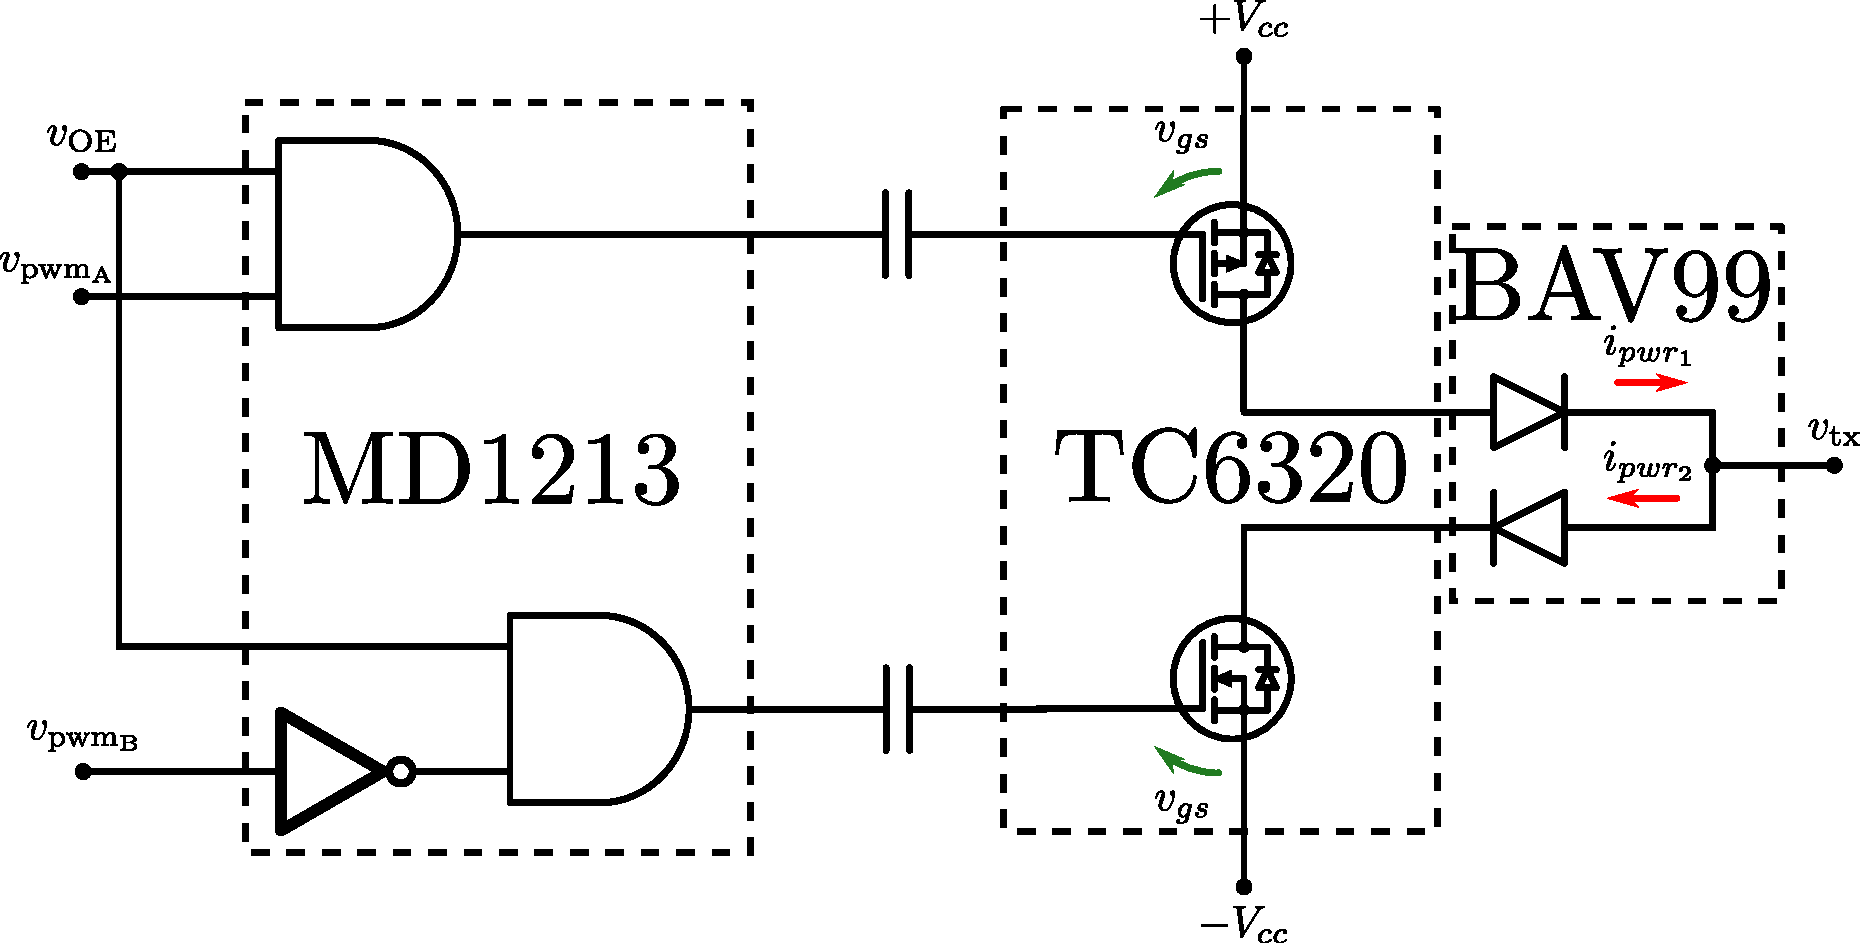
\includegraphics[width=\textwidth]{circuits/power_stage.pdf}
	\label{fig:3_power_stage}
	\caption{Circuit diagram of power stage}
\end{figure}
Gate drivers \cite{ISL55111,MD1213,EL7104}

\section{Transmit/Receive Switch}
\begin{figure}[htbp]
	\centering
	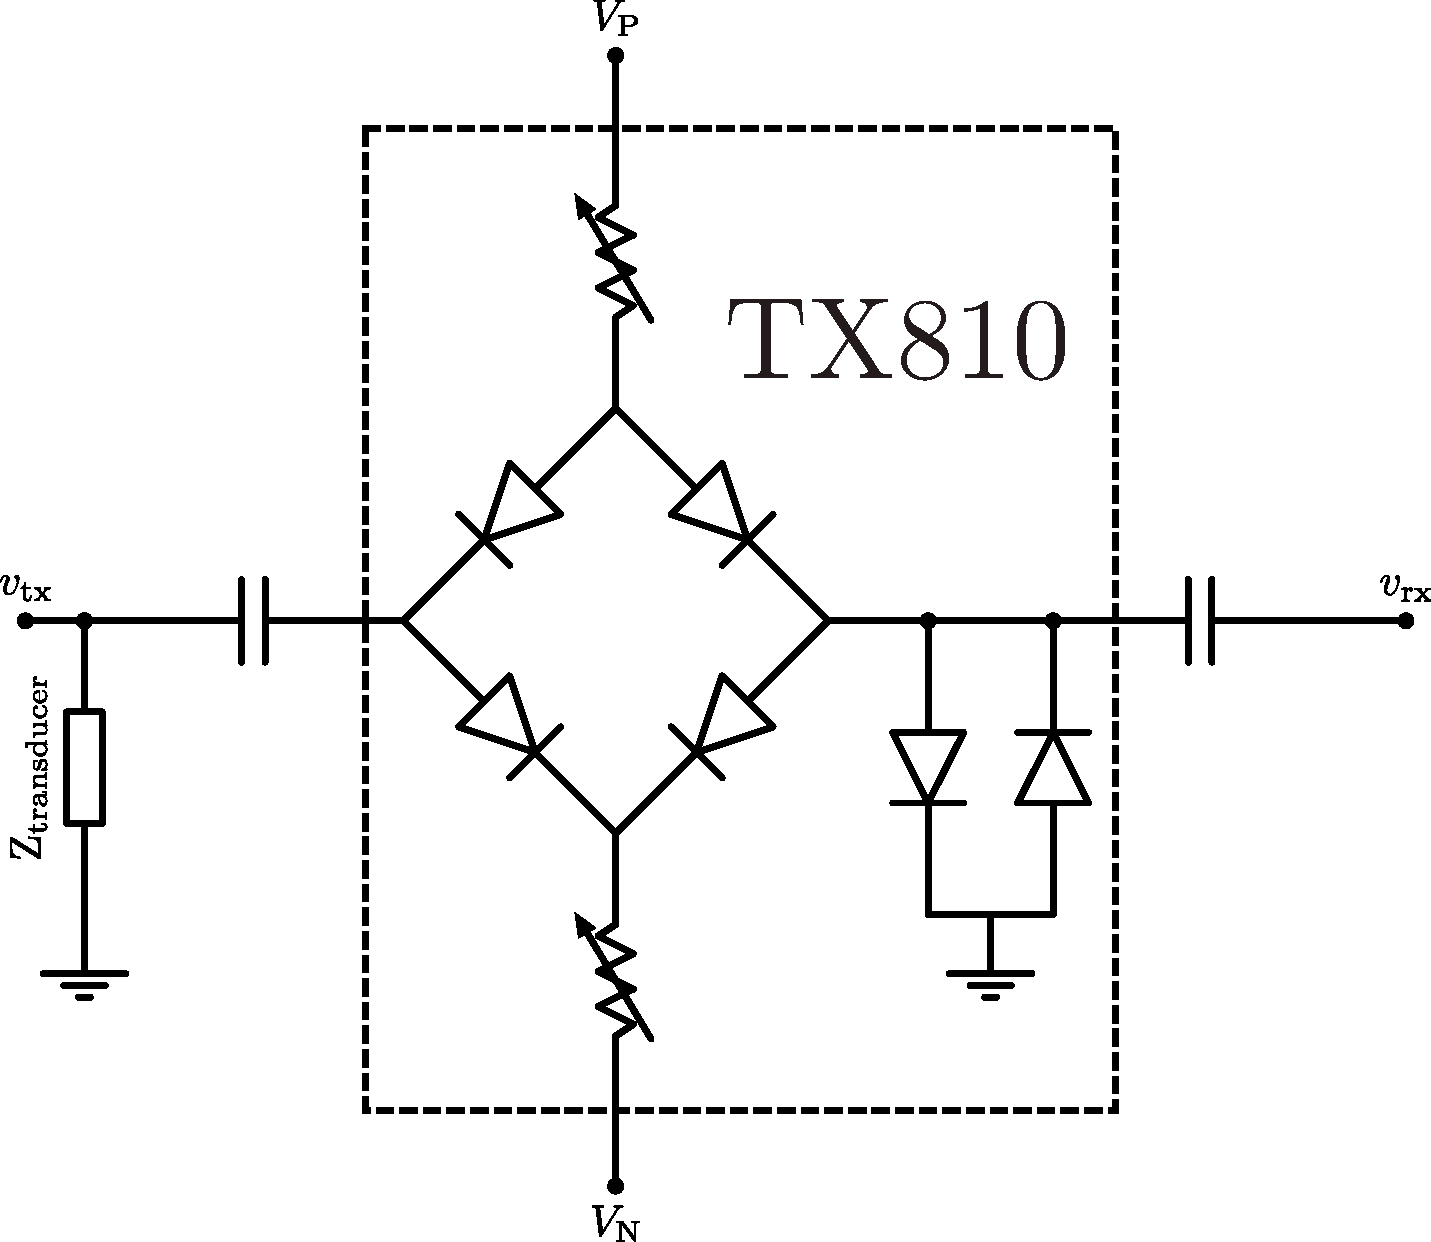
\includegraphics[width=.6\textwidth]{circuits/switch.pdf}
	\label{fig:3_switch}
	\caption{Circuit diagram of switch (per channel)}
\end{figure}
The transmit/receive switch is a module that is based on an IC from Texas Instruments known as TX810\cite{TX810}. The TX810 is an electronic device that can be used to switch transmit and receive paths of an ultrasound system. It can switch the transmit and receive paths for up to 8 different transducers (also known as probes) at the same time. The TX810 is programmed to switch the transmit and receive paths at specific times, as determined by the user. For example, the user can program the TX810 to switch the transmit and receive paths of a particular transducer at a specific time during the ultrasound examination. This allows the user to perform multi-channel imaging, where multiple transducers are used simultaneously to capture images from different angles. The IC is typically used in conjunction with an ultrasound system and one or more transducers. Transducers are used to transmit and receive ultrasound waves, which are used to generate images of the body's internal structures. The TX810 is used to switch the transmit and receive paths for each transducer at the appropriate times, allowing the ultrasound system to capture images from multiple angles simultaneously. When high-voltage transmitter signals are applied to the input, the internal diodes limit the output voltage. While in receive mode, the TX810's insertion loss is minimized. The TX810 features a 3-bit interface that may be used to program bias current from \qty{7}{\milli\ampere} to \qty{0}{\milli\ampere} for varying performance and power requirements, unlike conventional T/R switches. The device is put up in power-down mode when the TX810 bias current is set to 0mA (high-impedance mode). The TX810 does not put significant load on high-voltage transmitters when operating in the high-impedance mode. The device can also wake up from power-down mode in less than a \unit{\micro\second}. These sophisticated programmable features enable systems to save a large amount of electricity. 

The module is designed with three channels available. That means three channels can be used, either three separate transducers for multi-angle sonography, or a \gls{cmut} with three channels in a single angle.

\section{Transducer}
Various \gls{transducer} types are used during the testing of this project. Initially, commercially available transducers were used in order to validate the experimental process of the pulse-echo and Doppler measurements. Commercially available transducers in this context means \gls{pzt} piezoe
\subsection{Impedance matching input}

\section{Preamplifier}
\subsubsection{OPA487}
The OPA847\cite{OPA847} is a high-performance, high-speed, voltage feedback amplifier with a bandwidth of over 1 GHz. It has a wide gain range, low distortion, and low noise, making it suitable for a variety of applications including video, RF, and high-speed data acquisition. The OPA847 has a single-ended input and a differential output, which allows it to be used in a variety of circuit configurations. It is available in a surface-mount package and operates over a wide supply voltage range.

\subsubsection{AD8332}
The AD8332\cite{AD8332} is a fully integrated, single-chip amplifier designed for use in a wide range of RF and microwave applications. It is a low-noise, high-linearity amplifier that can be used in a variety of configurations, including as a stand-alone amplifier or as part of a larger system. The AD8332 is a current-feedback amplifier that can operate over a wide frequency range, from 50 MHz to 4 GHz. It has a high level of integration, with all active components on a single monolithic IC. This makes it suitable for use in small form factor applications where space is at a premium. The AD8332 has a number of features that make it well-suited for use in RF and microwave applications. It has a high level of linearity, which allows it to amplify signals without introducing significant distortion. It also has a low noise figure, which makes it well-suited for use in low-noise applications. Additionally, the AD8332 has a wide dynamic range, which makes it capable of handling a wide range of input signals without clipping or saturating. Overall, the AD8332 is a versatile and reliable amplifier that can be used in a wide range of RF and microwave applications. It is well-suited for use in a variety of systems, including communication systems, radar systems, and instrumentation systems.

\section{Demodulation}
To demodulate our signal using the process described in The AD8333\cite{AD8333} is an integrated circuit (IC) that can be used to demodulate an amplitude-modulated (AM) signal. It contains all the necessary circuitry to detect and extract the information contained in an AM signal. In AM, the information is encoded in the amplitude of the carrier wave, which is modulated or varied in some way to convey the information. The AD8333 is able to detect these variations in the carrier wave and extract the original information from the signal. To do this, the AD8333 uses a process called envelope detection. It rectifies the input signal, which removes the negative portions of the waveform, and then filters the resulting signal to remove any remaining high-frequency components. This leaves only the envelope of the original modulated signal, which contains the encoded information. The AD8333 also includes amplifier and buffer stages to amplify the detected envelope and prepare it for further processing or application. It is often used in radio communication systems, industrial control systems, and other applications where an AM signal needs to be demodulated and the information contained in the signal needs to be extracted. Test af git push.
\section{Sample/Hold}
Sample and hold
\section{Pulse-Repetition and Wall Filter}

\section{Amplifier}

\section{Mixer}

\section{Adder}